% !TEX root = ../main.tex

\section{Experimental measurements}

Reactor measurements from fast pyrolysis experiments of the Blend3 and forest residue feedstocks are provided in this section. Chemical analysis and size characterization data are also given for each feedstock.

\subsection{Blend3 feedstock}

EFR operating conditions related to the Blend3 feedstock such as temperatures, pressures, and flow rates are shown in Figure \ref{fig:efr-blend3}. Nitrogen gas at 500$^{\circ}$C (773.15 K) is generally used as the conveying medium for the feedstock material.

\begin{figure}[H]
    \centering
    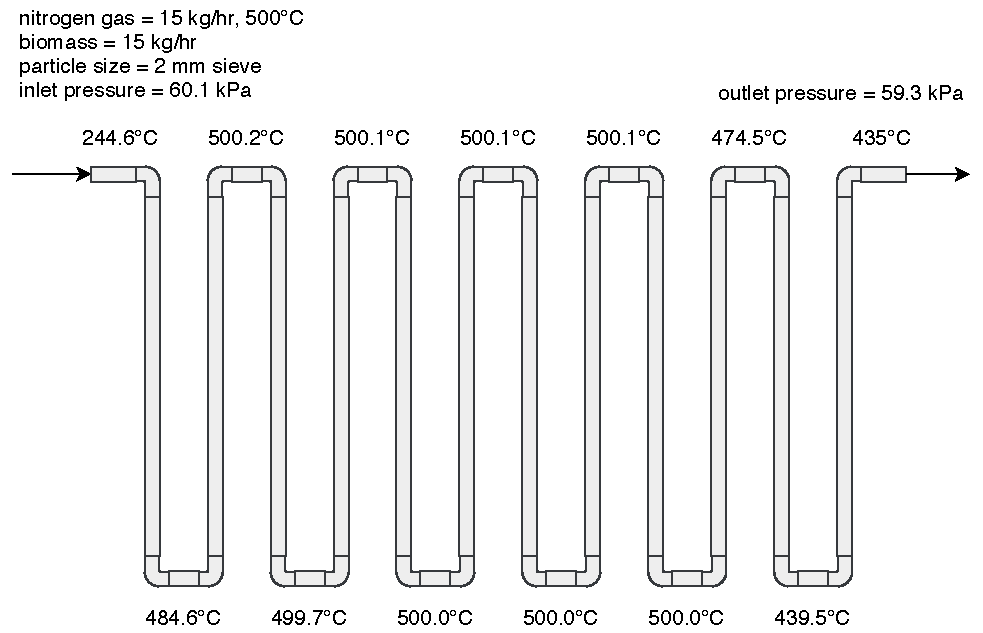
\includegraphics[width=\textwidth]{figures/efr-blend3.pdf}
    \caption{Operating conditions for the Blend3 feedstock in the EFR. Pressure is reported as gauge pressure. Data provided by NREL.}
    \label{fig:efr-blend3}
\end{figure}

Proximate and ultimate analysis data for the Blend3 feedstock are presented in Tables \ref{tab:blend3-prox} and \ref{tab:blend3-ult}. Only one set of analysis data is available therefore the uncertainty in the values is unknown. Ideally, three sets of measurements would be conducted to give confidence in the reported data.

\begin{table}[H]
    \centering
    \caption{Blend3 proximate analysis mass percent, as-received basis. Source \cite{Choratch-2017}.}
    \label{tab:blend3-prox}
    \begin{tabular}{lrrr}
        \toprule
        Proximate & \% ar & \% ar & \% ar \\
        \midrule
        FC        & 16.92 & ? & ? \\
        VM        & 76.40 & ? & ? \\
        ash       & 0.64  & ? & ? \\
        moisture  & 6.04  & ? & ? \\
        \bottomrule
    \end{tabular}
\end{table}

\begin{table}[H]
    \centering
    \caption{Blend3 ultimate analysis mass percent, as-received basis. Source \cite{Choratch-2017}.}
    \label{tab:blend3-ult}
    \begin{tabular}{lrrr}
        \toprule
        Element & \% ar & \% ar & \% ar \\
        \midrule
        C        & 49.52   & ? & ? \\
        H        & 5.28    & ? & ? \\
        O        & 38.35   & ? & ? \\
        N        & 0.15    & ? & ? \\
        S        & 0.02    & ? & ? \\
        ash      & 0.64    & ? & ? \\
        moisture & 6.04    & ? & ? \\
        \bottomrule
    \end{tabular}
\end{table}

The chemical analysis of the Blend3 feedstock is presented in Table \ref{tab:blend3-chem-analysis}. Again, only one set of data is available so the uncertainty in the measurements is unknown. The chemical analysis measurements are used to determine the biomass composition which is needed for the kinetics model. Ash analysis is given in Table \ref{tab:blend3-ash-analysis} while particle properties are provided in Table \ref{tab:blend3-properties}.

\begin{table}[H]
    \centering
    \caption{Blend3 chemical analysis mass percent, dry basis. Source \cite{Starace-2020}.}
    \label{tab:blend3-chem-analysis}
    \begin{tabular}{lrrr}
        \toprule
        Chemical component & \% dry & \% dry & \% dry \\
        \midrule
        glucan                    & 38.95 & ? & ? \\
        acetyl                    & 1.59  & ? & ? \\
        arabinan                  & 1.40  & ? & ? \\
        galactan                  & 3.16  & ? & ? \\
        mannan                    & 10.52 & ? & ? \\
        xylan                     & 7.89  & ? & ? \\
        lignin                    & 29.48 & ? & ? \\
        free fructose             & 0.07  & ? & ? \\
        free glucose              & 0.04  & ? & ? \\
        sucrose                   & 0.04  & ? & ? \\
        water extractives         & 2.75  & ? & ? \\
        ethanol extractives       & 3.49  & ? & ? \\
        non-structural inorganics & 0.22  & ? & ? \\
        structural inorganics     & 0.41  & ? & ? \\
        \bottomrule
    \end{tabular}
\end{table}

\begin{table}[H]
    \centering
    \caption{Blend3 ash analysis as weight percent of ash. Source \cite{Choratch-2017}.}
    \label{tab:blend3-ash-analysis}
    \begin{tabular}{lrrr}
        \toprule
        Metal oxide & wt. \% & wt. \% & wt. \% \\
        \midrule
        SiO$_2$     & 28.1 & ? & ? \\
        Al$_2$O$_3$ & 7.06 & ? & ? \\
        TiO$_2$     & 0.34 & ? & ? \\
        CaO         & 21.8 & ? & ? \\
        Na$_2$O     & 0.71 & ? & ? \\
        K$_2$O      & 13.8 & ? & ? \\
        P$_2$O$_5$  & 5.47 & ? & ? \\
        SO$_3$      & 1.23 & ? & ? \\
        Cl          & 0.09 & ? & ? \\
        CO$_2$      & 5.14 & ? & ? \\
        \bottomrule
    \end{tabular}
\end{table}

\begin{table}[H]
    \centering
    \caption{Blend3 particle properties from pelletized crushed feedstock. The crushed feedstock is used in the entrained flow reactor.}
    \label{tab:blend3-properties}
    \begin{tabular}{crlc}
        \toprule
        Property & Value & Description & Source \\
        \midrule
        $\rho$  & 1,050 kg/m$^3$ & particle density, daf basis & \cite{Pecha-2018} \\
        $\eta$  & 0.27           & particle porosity & \\
        $k$     & 0.23 W/mK      & thermal conductivity & \\
        \bottomrule
    \end{tabular}
\end{table}

Pyrolysis yields expected from the entrained flow reactor for the Blend3 feedstock are listed in Table \ref{tab:blend3-efr-yields}. Char is assumed to be the total solids in the reactor which includes un-pyrolyzed or partially-pyrolyzed biomass particles. Total liquid is considered to be the tar or bio-oil yield generated from the pyrolysis process.

\begin{table}[H]
    \centering
    \caption{Entrained flow reactor yields for Blend3 feedstock.}
    \label{tab:blend3-efr-yields}
    \begin{tabular}{lr}
        \toprule
        Yield & wt. \% \\
        \midrule
        total liquid   & 64.9 \\
        char           & 13.9 $\pm$ 0.1 \\
        gas            & 17.2 $\pm$ 0.2 \\
        mass balance   & 96.9 $\pm$ 1.5 \\
        carbon balance & 93.0 $\pm$ 1.0 \\
        \bottomrule
    \end{tabular}
\end{table}

\subsection{Forest residue feedstock}

The forest residue feedstock is comprised of branches/twigs, cambium, needles, bark, and whitewood. This feedstock is used in the NREL fluidized bed reactor (FBR) for the purposes of the FCIC project. The FBR is operated at fast pyrolysis conditions for the thermochemical conversion of biomass. The reactor is sometimes referred to as the 2FBR.

\begin{table}[H]
    \centering
    \caption{General information for the forest residue feedstock.}
    \begin{tabular}{ll}
        \toprule
        Item    & Description \\
        \midrule
        Name    & forest residue \\
        ID      & ? \\
        Contact & ? \\
        \bottomrule
    \end{tabular}
\end{table}

\begin{table}[H]
    \centering
    \caption{Bark ultimate analysis mass percent, dry ash-free basis. Source \cite{Unknown-2019}.}
    \begin{tabular}{lrrr}
        \toprule
        Element & \% daf & \% daf & \% daf \\
        \midrule
        C        & 48.27 & ? & ? \\
        H        & 5.72  & ? & ? \\
        N        & 0.52  & ? & ? \\
        \bottomrule
    \end{tabular}
\end{table}

\begin{table}[H]
    \centering
    \caption{Branches/twigs ultimate analysis mass percent, dry ash-free basis. Source \cite{Unknown-2019}.}
    \begin{tabular}{lrrr}
        \toprule
        Element & \% daf & \% daf & \% daf \\
        \midrule
        C        & 49.69 & ? & ? \\
        H        & 6.36  & ? & ? \\
        N        & 0.25  & ? & ? \\
        \bottomrule
    \end{tabular}
\end{table}

\begin{table}[H]
    \centering
    \caption{Cambium ultimate analysis mass percent, dry ash-free basis. Source \cite{Unknown-2019}.}
    \begin{tabular}{lrrr}
        \toprule
        Element & \% daf & \% daf & \% daf \\
        \midrule
        C        & 48.52 & ? & ? \\
        H        & 6.39  & ? & ? \\
        N        & 0.11  & ? & ? \\
        \bottomrule
    \end{tabular}
\end{table}

\begin{table}[H]
    \centering
    \caption{Needles ultimate analysis mass percent, dry ash-free basis. Source \cite{Unknown-2019}.}
    \begin{tabular}{lrrr}
        \toprule
        Element & \% daf & \% daf & \% daf \\
        \midrule
        C        & 48.59 & ? & ? \\
        H        & 5.92  & ? & ? \\
        N        & 1.22  & ? & ? \\
        \bottomrule
    \end{tabular}
\end{table}

\begin{table}[H]
    \centering
    \caption{Whitewood ultimate analysis mass percent, dry ash-free basis. Source \cite{Unknown-2019}.}
    \begin{tabular}{lrrr}
        \toprule
        Element & \% daf & \% daf & \% daf \\
        \midrule
        C        & 48.27 & ? & ? \\
        H        & 6.15  & ? & ? \\
        N        & 0.10  & ? & ? \\
        \bottomrule
    \end{tabular}
\end{table}

\begin{table}[H]
    \centering
    \caption{Whitewood biomass composition mass percent, dry basis. Source \cite{Unknown-2020}.}
    \begin{tabular}{lr}
        \toprule
        Component & \% dry \\
        \midrule
        Cellulose       & 38.04 \\
        Hemicellulose   & 24.2  \\
        \bottomrule
    \end{tabular}
\end{table}
